\documentclass[12pt,letterpaper,boxed]{hmcpset}
\usepackage{float}
\restylefloat{figure}
\usepackage{graphicx}
\usepackage{amsmath}


\name{Lujia Zhang}
\class{CSSE 477}
\mailbox{CM 1405}
\assignment{Lab4}

\begin{document}

\begin{problem}[1. What is the job of Compute and Task interfaces?.]
\end{problem}

The Compute interface provides a framework for the server to execute and respond to the task.
The Task interface provides a framework for a client to submit a task to a server. \newline \newline
\begin{problem}[2. The Compute interface extends the Remote interface but the Task interface does not. When a client creates these objects, explain how they get sent to the server? [Hint: Slide\# 9].]
\end{problem}

In the Client, the broker, or the Registry, finds the compute class based on the agruments given at runtime. Then, in order to compute a task, the client creates a Pi object, which implements the Task interface. Then the compute class calls executeTask on the Pi object. \newline \newline
\begin{problem}[3. Which object is equivalent to a Broker (of the Broker Architecture) in ComputeEngine and why?]
\end{problem}

java.rmi.registry.Registry because it is in charge of storing servers (line 75-78 in ComputeEngine) and looking them up (line 65 in ComputePi).
\newline \newline
\begin{problem}[4. When a client gets hold of a stub of ComputeEngine, which method of the class will be remotely called by the client?]
\end{problem}

The executeTask method. \newline\newline
\begin{problem}[5. List all of the high-level steps involved in creating a RMI server object.]
\end{problem}

The server needs to register itself with the registry by creating a stub from a new instance of that class. Then the server is then mapped to some string determined by the class. \newline\newline\newline
\begin{problem}[6. List all of the high-level steps involved in creating a RMI client.]
\end{problem}

The client just needs to connect to the registry and pull the server with the string key \newline\newline
\begin{problem}[7. Why is the PI class implementing both Task and Serializable interfaces]
\end{problem}

So it can be broken down, sent over the network, and re-established. \newline \newline
\begin{problem}[Screen shot of Running the RMI Client]
\end{problem}
\begin{figure}[H]
  \centering
  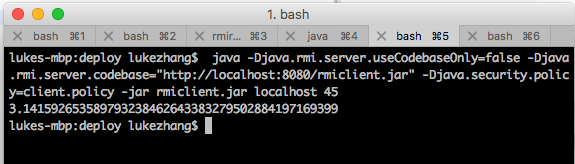
\includegraphics[width = 1.0\textwidth]{1.png}
\end{figure}
\begin{problem}[Screen shot of Running with other winodws machine, prime number]
\end{problem}
\begin{figure}[H]
  \centering
  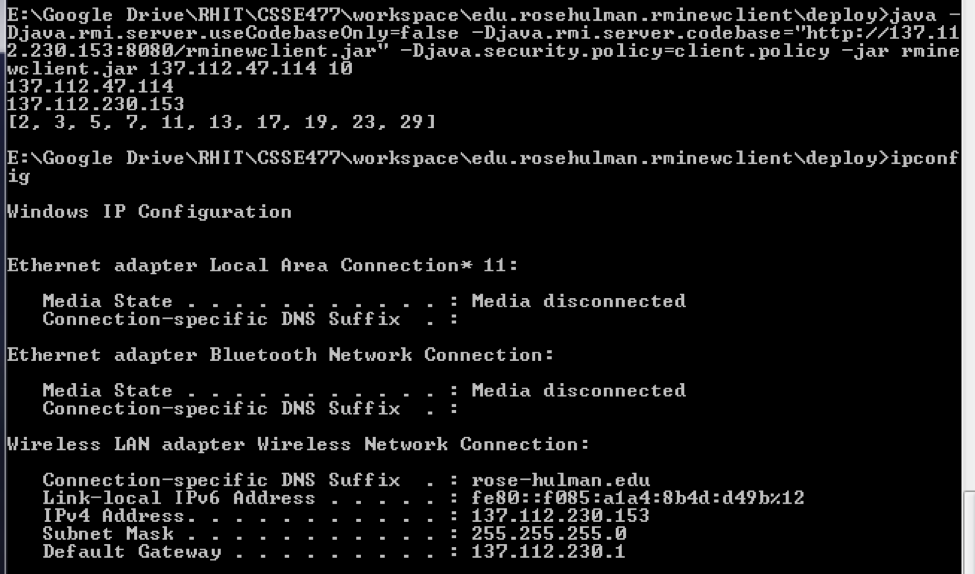
\includegraphics[width = 1.0\textwidth]{2.png}
\end{figure}
\end{document}